\documentclass[a4paper]{article}

\usepackage{INTERSPEECH2018}
\usepackage{booktabs}
\usepackage{adjustbox}
\usepackage{multirow}
\usepackage{textcomp}
\usepackage{caption}
\usepackage{subcaption}

\title{Multilingual Multi-Task Learning for Low-Resource Acoustic Modeling}

\name{Josh Meyer$^1$}
%The maximum number of authors in the author list is twenty. If the number of contributing authors is more than twenty, they should be listed in a footnote or in acknowledgement section, as appropriate.
\address{
  $^1$University of Arizona}
\email{joshua.richard.meyer@gmail.com}

\begin{document}

\maketitle
% 
\begin{abstract}
  The following study investigates low-resource multilingual acoustic model training with Multi-Task Learning (MTL) for Automatic Speech Recognition. The main question of this research is: \textit{What is the best way to represent a source language with MTL to improve performance on the target language?} The two parameters of interest are (1) the level of detail at which the source language is modeled, and (2) the relative weighting of languages during backprop.

  I found that when the source task is weighted higher than the target task, a lower level of source task representation (ie. the triphone) leads to better performance in the target language.  On the other hand, when the target task is weighted heavier than the source task, then a more abstract level of source task representation (ie. the monophone) is better for performance in the target language. I found that a 1-to-1 weighting ratio of source-to-target leads to best results on average.

\end{abstract}

\noindent\textbf{Index Terms}: speech recognition, multi-task learning, acoustic modeling





\section{Introduction}

Performance for a low-resource language on speech recognition can be improved by adding training data from another, resource-rich language. Typically, data from another language is added as a separate task in the Multi-Task Learning (MTL) framework  \cite{caruana1997} via an additional output layer. The targets for this addititional language have typically been states of context-dependent triphones, defined by some tree clustering algorithm \cite{huang2013,heigold2013,grezl2016}.

MTL should work in situations where the tasks are related. For example, recognizing the presence of a tail helps recognize the location of a cat in an image, because tails are highly predictive of cats, and vice versa. By forcing a neural net to recognize cats and tails in the same image, the hidden layers will be biased towards more generalizable, task-independent representations of the data.

Cats and tails are obviously related, but it is difficult to  automatically identify related tasks for a new classification problem. The current study investigates the effectiveness of auxiliary tasks which are not hand-crafted by an expert, but rather extracted from a stage in the traditional ASR pipeline (ie. the Hybrid DNN-HMM pipeline). The traditional pipeline includes model transfer, where the labels are defined by a decision tree. This decision tree models fine-grained contextual information which is language-specific, and gets more fine-grained further down the tree. The leaves of this tree model what are called context-dependent triphones.

This current research builds off the intuition that these triphones encode information which is very specific to the source language, and maybe not the best representation for language-transfer. Using a higher-level of linguistic abstraction (ie. states closer to the roots of the tree), we extract more language-general information. Another aspect of MTL which effects training is the relative weighting of the source task to the target task during backprop. If the tasks come from separate datasets, the task with the most training examples will have most influence during backprop. 

The following experiments show that both the level of detail and the relative weighting of the source language is important for MTL. These two factors (source task weighting and detail) interact such that, to acheive best results, a more detailed task should be weighted more, and a less detailed task should be weighted less. After an analysis of performance on training and validation data, we see that less detailed (ie. more simple) tasks are easier to learn, and as such, they find a good local minumum quickly and don't budge from that place. However, this local minimum may not be best for the target task.

In the following experiments, the simple auxiliary task labels are monophones and the complex auxiliary task labels are triphones. An intermediate level of abstraction (which I dub the ``half-phone'') is also investigated. Relative weighting schemes for target-to-source data are the following: 1-to-2, 1-to-1, and 2-to-1. The triphone task performed best with 1-to-2 weighting, the half-phone performed best with 1-to-1 weighting, and the monophone performed best with 2-to-1 weighting. The addition of multiple auxiliary tasks resulted in lower accuracies.

The target language is Kyrgyz, and the source language is English. Both data come from audiobooks, English from LibriSpeech \cite{panayotov2015} and Kyrgyz from the Bizdin.kg project.




\section{Background}

Past work on MTL for acoustic modeling can be divided into two main categories: monolingual or multilingual. Multilingual MTL acoustic modeling involves training a single DNN with multiple output layers, where each output layer represents triphones from one language. Monolingual MTL acoustic modeling involves designing multiple tasks for a single language, where each task is linguistically relevant (eg. triphones vs. monophones vs graphemes). 

The earliest examples of MTL with multiple languages can be found in \cite{huang2013} and \cite{heigold2013}, who both used triphones from each language as additional tasks. They were interested in improving performance on all languages, not just one target language. More recently, \cite{grezl2016} found that increasing number of triphones and amount of data from a single source language leads to better performance in some low-resourced language.


With regards to monolingual MTL, research has aimed to find tasks (from the same language) which are phonetically relevant to the main task. Both \cite{seltzer2013} and later \cite{huang2015} looked at a very similar approach to what I explore here, with MTL on broader, more abstract phonetic categories for English. They both found improvement on TIMIT, but they didn't investigate multilingual transfer. With regards to low-resource languages, \cite{chen2014} and later \cite{chen2015} similarly looked at MTL for a single target language, using graphemes or a universal phoneset as extra targets.



\section{DNN-Hybrid Training as Model Transfer}

The standard DNN-Hybrid approach requires the GMM-HMM system to provide the labels for supervised training. This reliance of the DNN on GMM alignments is actually a form of model transfer, where the DNN is trained to perform the extact same classification as its GMM predecessor. The DNN not only learns the frame alignments from the individual GMMs, but also the structure of the phonetic decision tree used to define the labels. The output layer of the DNN is trained to predict targets which were defined via leaves of the decision tree, as is shown in Figure (\ref{fig:tree-net})\footnote{The original decision tree graphic comes from \cite{young2002}, and the original neural net graphic comes from \cite{heigold2013}}.


\begin{figure}[!htbp]
  \centering
\minipage{0.5\textwidth}
  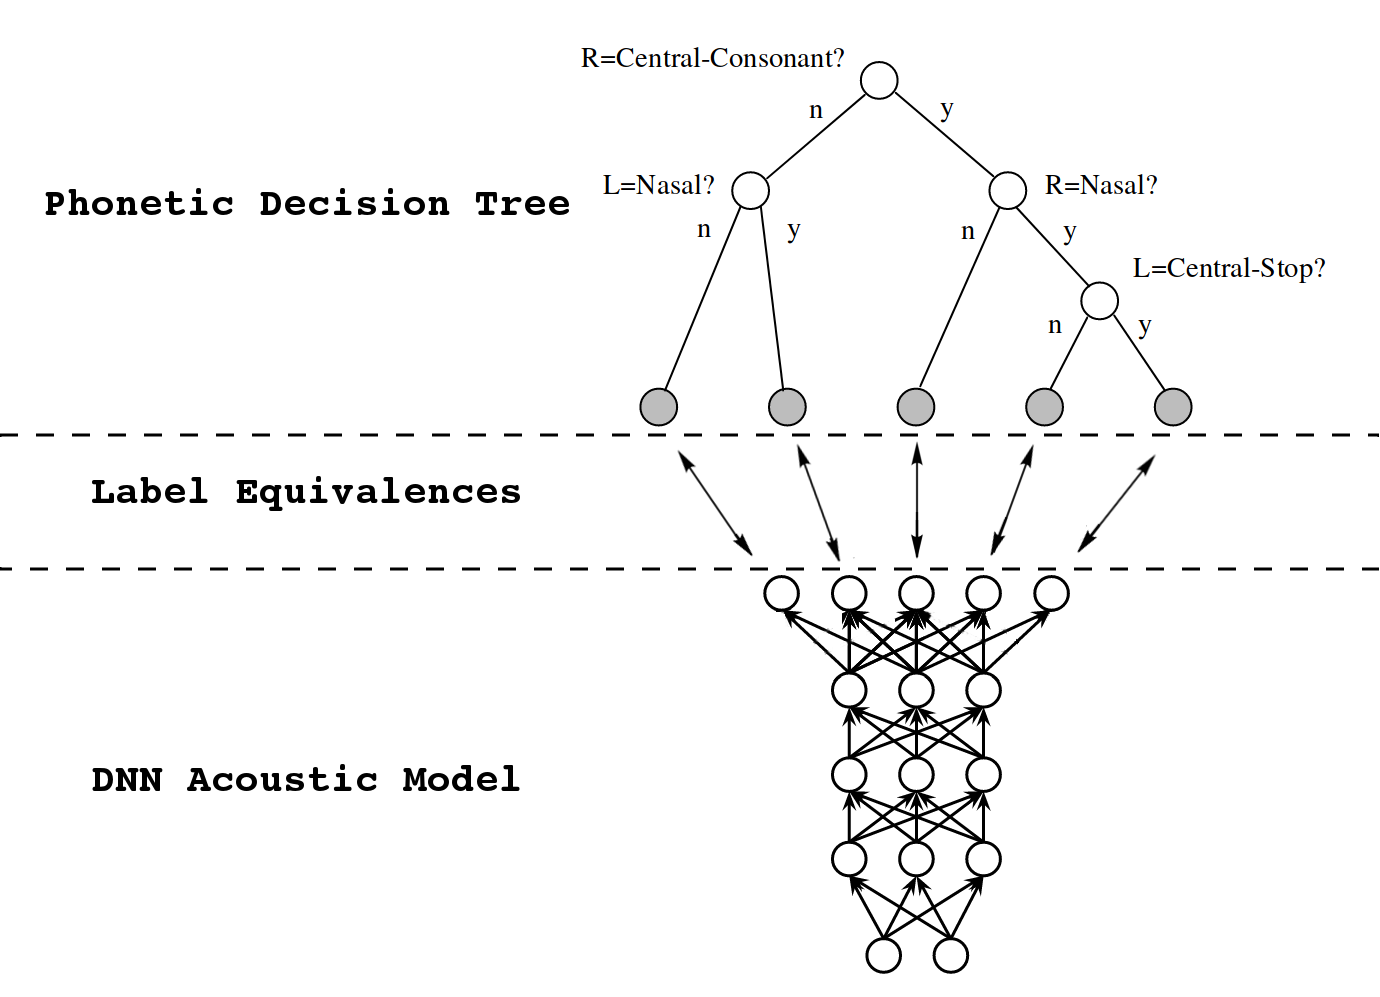
\includegraphics[width=\linewidth]{figs/tree-net.png}
  \caption{GMM$\rightarrow$DNN Model Transfer}
    \label{fig:tree-net}
  \endminipage\hfill
\end{figure}

In this model transfer approach, all the heirarchical knowledge inherent to the decision tree is lost to the DNN. The DNN only sees the leaves of the tree, but none of the relationships among those leaves. That is, the branches and roots are lost, which main contain important, language-general knowledge. The current study extracts the heirarchical knowledge of this tree via MTL, by modeling various levels of the tree as separate tasks. 


\section{Experiments}

The following experiments tease out (1) the level of detail at which the source language should be modeled and (2) the amount of weighting which should be given to the target language training examples.

The first point of interest is the level of detail at which the source language is modeled. This is investigated via addition of multiple tasks to the TDNN during training. The experiements here are crafted to answer the question: \textit{How much phonetic detail should the source language be modeled at to best transfer inductive bias to the target language?}

We can model the source language with lots of contextual detail (ie. the triphone), with abstracted, context-independent detail (ie. the monophone), or somewhere in between. Building of the traditional hybrid DNN-HMM ASR training pipeline, investigating these levels of representation are easily acheived via the phonetic decision tree (cf. Figure (\ref{fig:tree-parts})\footnote{Original figure from \cite{young2002}.}). We can merely assign labels to training data frames by moving up the tree, from leaves (triphones) to roots (monophones).

The second point of interest is the relative weighting of target vs. source language training data. It is clear that if we train two languages in parallel, the source language (with many more training samples) will dominate the target language in the fight for influence over shared hidden layers during backprop.

To my knowledge, the importance of relative weighting has not been investigated in ASR acoustic modeling (although it was dedicated its own chapter in Caruana's 1997 dissertation \cite{caruana1997}). To investigate weighting further, I examine the following target vs. source weighting schemes: 1-to-2, 1-to-1, and 2-to-1 (all ratios are target-to-source).

These weights are instantiated during training via a weight to the target output label, where the label is a one-hot vector. For example, given 1000 hours of source language and 1 hour of target language, to acheive a 1-to-1 ratio in training, I would multiply the target labels from the target language by 1000, resulting in target vectors such as \texttt{$[0, 0, 0, 0, 1000, 0, 0, \ldots]$} instead of \texttt{$[0, 0, 0, 0, 1, 0, 0, \ldots]$}.



\subsection{Data}

Two speech corpora are used in the following experiments:

\begin{enumerate}
\item $\approx$ 5 hours of English (4.86 hours of LibriSpeech)
\item $\approx$ 1.5 hours of Kyrgyz (1.59 hours of audiobook)
\end{enumerate}

\subsection{Model Building}

All models were build using the Kaldi toolkit as Time-Delay Neural Networks (TDNNs) via the \texttt{nnet3} approach \cite{povey2011,peddinti2015}. The main neural net run script used in this paper can be found at www.github.com/JRMeyer/kaldi-mirror/egs/kgz/kyrgyz-model/run\_nnet3\_multilingual.sh. The main GMM script used to create data alignments can be found at www.github.com/JRMeyer/kaldi-mirror/egs/kgz/kyrgyz-model/run\_gmm.sh.

In GMM training, monophones (for each language) were allotted 1,000 Gaussian components, and trained over 25 iterations of EM. These monophones were then expanded into context-dependent triphones via a phonetic decision tree, with a maximum of 2,000 leaves \& 5,000 Gaussians (LibriSpeech reached 1584 leaves, and Kyrgyz reached 752). The resulting tied-state clusters (ie. leaves) are then trained as context-dedendent triphones over 25 iterations of EM.

Given the alignments from the GMM-HMM models, a 5-layer, 500-dimensional TDNN is trained over 10 epochs of backprop on a single GPU instance.

Each auxiliary task is implemented as a separate output layer along with a separate, penultimate hidden layer. All other hidden layers of the TDNN are trained in parallel. A declining learning rate was used, with an initial $\alpha_{initial}=0.0015$ and a final $\alpha_{final}=0.00015$. The objective function is $max( KaldiBatchNorm(ReLU\_activation) \bullet target )$.

During testing, \textit{only} the main task is used. The additional tasks are dropped and the baseline Kyrgyz triphones are used in decoding. This highlights the purpose of the extra tasks: to force the learning of robust representations in the hidden layers during training; they serve as ``training wheels'' which are then removed once the net is ready.



\subsubsection{Baseline Model}

All the following architectures will be compared to the performance of a baseline model of identical architecture (5 hidden layers, 500-dimentional layers, ReLU activations, same training algorithm). The output targets are standard context-dependent triphones trained on Kyrgyz audio.

To account for any advantage mutliple output layers may bring about, the baseline contains two output layers, where the tasks are identical. In this way, random initializations in the weights and biases for each task are accounted for.

\subsubsection{Auxiliary Tasks}

The auxiliary tasks all train on English language data from the LibriSpeech corpus. Investigating the intuition that labels generated by a standard triphone phonetic decision tree are not the best representation of data for transfer learning, the auxiliary tasks here investigate different levels in the decision tree's branches.

I split the LibriSpeech phonetic decision tree into three logical parts, shown in Figure (\ref{fig:tree-parts}):

\begin{enumerate}
\item roots (standard monophones)
\item branches (what I dub, ``half''-phones)
\item leaves (standard triphones)
\end{enumerate}




\begin{figure}[!htbp]
  \centering
\minipage{0.525\textwidth}
  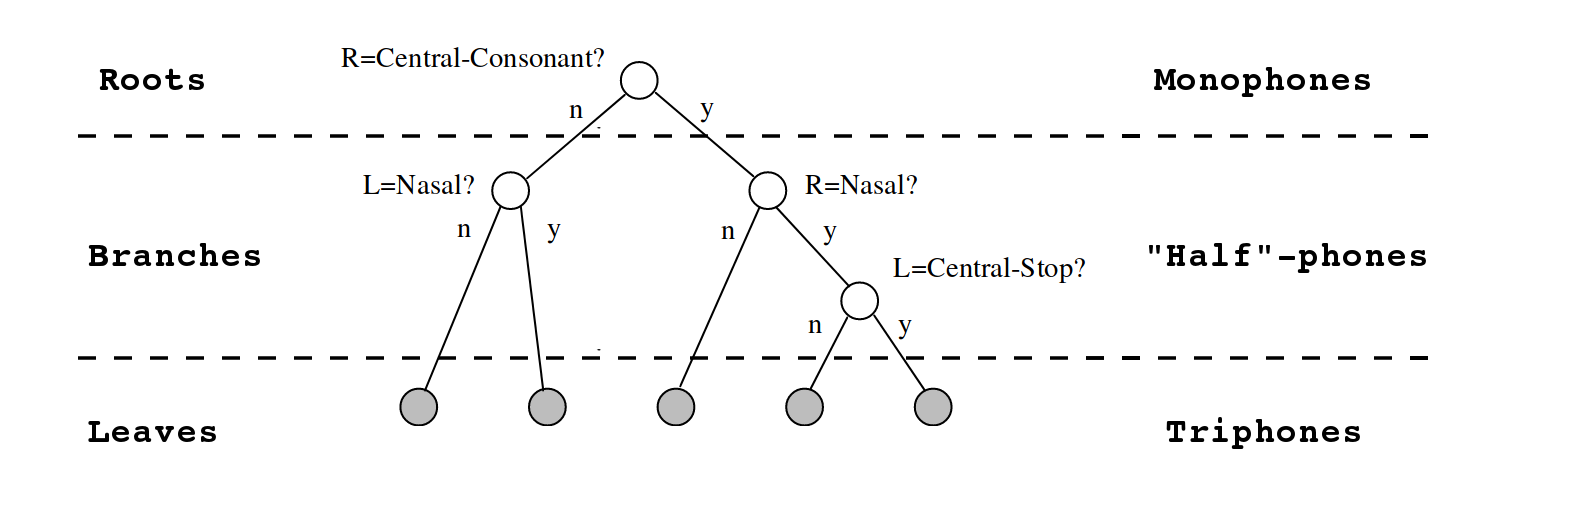
\includegraphics[width=\linewidth]{figs/levels.png}
  \caption{Logical Tree Parts}
  \label{fig:tree-parts}
\endminipage\hfill
\end{figure}


The ``half''-phones were created by halving the optimal number of leaves from the triphone system (ie. 1584 leaves) and re-training a new GMM-HMM system with half the optimal number of leaves (1/2 * 1584 = 792 leaves). All the other parameters were left unchanged (number of Gaussian components, iterations of EM, etc.). An overview of the auxiliary tasks can be found in Table (\ref{tab:tasks}).




\begin{table}[!htbp]
  \centering
  \caption{Auxiliary Tasks}
  \label{tab:tasks}
  \begin{adjustbox}{width=.45\textwidth}
    \begin{tabular}{lcc}
      \toprule
      \textbf{Logical Tree Part} & \textbf{Level of Phonetic Detail} & \textbf{ \textnumero~of Tasks}\\
      \midrule
      Roots & Monophones & 1\\
      Branches & Half-phones & 1\\
      Leaves & Triphones & 1\\ 
      Lower Tree & Monophones + Half-phones & 2\\
      Upper Tree & Half-phones + Triphones & 2\\
      Whole Tree & Monophones + Half-phones + Triphones & 3\\
      \bottomrule
    \end{tabular}
  \end{adjustbox}
\end{table}

By forcing the neural net to recognize higher levels in the English source tree, we will learn representations which are more abstract, and therefore more likely to be relevant multi-lingually. 


\subsubsection{Weighting Procedure}

The addition of each above task adds approximately 5 hours of training data to the standard training of a Single Task Model on Kyrgyz. As such, a weighting procedure was used to balance the relative influence of source vs. target training data on backprop. For example, to reach a one-to-one ratio, where one hour of Kyrgyz is equal to one hour of English, I multiplied every Kyrgyz target one-hot vector by $3.06$. The exact weighting scheme is shown in Table (\ref{tab:weights}).

\begin{table}[!htbp]
  \centering
  \caption{Target:Source Data Weighting Scheme}
  \label{tab:weights}
  \begin{adjustbox}{width=.3\textwidth}
    \begin{tabular}{cc}
      \toprule
      \textbf{Target:Source Ratio} & \textbf{Target Weighting}\\
      \midrule
      1:2 & 1.53x  \\
      1:1 & 3.06x  \\
      2:1 & 6.12x  \\
      \bottomrule
    \end{tabular}
  \end{adjustbox}
\end{table}




\subsection{Results}


All results are performed on the same held-out section of Kyrgyz audiobook. The bigram language model, lexicon, and main-task decision tree are built into a standard decoding graph in the traditional Kaldi TDNN pipeline. Decoding is performed with a bigram backoff language model trained on a Wikipedia Kyrgyz dump, and contains, 103,998 unigrams and 56,6871 bigrams.

The experimental results are shown in Table (\ref{tab:results}) as percent Word Error Rate (WER) relative to the baseline model. All experiments show improvement over the baseline.

\begin{table}[!htbp]
  \centering
  \caption{Word Error Rates (WER\%) Relative to Baseline}
    \label{tab:results}
  \begin{adjustbox}{width=.45\textwidth}
    \begin{tabular}{lccc}
      \toprule
      & \multicolumn{3}{c}{\textbf{Target:Source Weighting}} \\
      \textbf{Auxiliary (Source Lang) Tasks} & \textit{1-to-2} & \textit{1-to-1} & \textit{2-to-1}\\
      \midrule
      STL Baseline                          &  \multicolumn{3}{c}{50.54\% WER}  \\
      Monophones                            &  -3.13  & -3.22 & \textbf{-2.34}  \\
      Halfphones                            &  -1.86  & \textbf{-3.81} & -1.86 \\
      Triphones                             &  \textbf{-3.81} & -3.42 & -1.17  \\
      Monophones + Halfphones               &  -2.44  & -2.05 &  \textbf{-2.34}\\
      Halfphones + Triphones                &  -2.64  & -2.54 & -0.49 \\
      Monophones + Halfphones + Halfphones  &  -1.95  & -2.34 &  -1.66\\
      \midrule
      AVERAGE                               &  -2.64  & -2.90 & -1.64 \\
      \bottomrule
    \end{tabular}
  \end{adjustbox}
\end{table}


%% \begin{table}[!htbp]
%%   \centering
%%     \caption{TDNN // 5-layer // 500-dim //  10 epoch }
%%   \begin{adjustbox}{width=.45\textwidth}
%%     \begin{tabular}{lccc}
%%       \toprule
%%       & \multicolumn{3}{c}{\textbf{Target:Source Weighting}} \\
%%       \textbf{Auxiliary (Source Lang) Tasks} & \textit{1-to-2} & \textit{1-to-1} & \textit{2-to-1}\\
%%       \midrule
%%       STL Baseline                          &  \multicolumn{3}{c}{50.54}  \\
%%       Monophones                            &  47.41  & 47.32 & 48.20  \\
%%       Halfphones                            &  48.68  & 46.73 & 48.68 \\
%%       Triphones                             &  46.73  & 47.12 & 49.37  \\
%%       Monophones + Halfphones               &  48.10  & 48.49 & 48.20 \\
%%       Halfphones + Triphones                &  47.90  & 48.00 & 50.05\\
%%       Monophones + Halfphones + Halfphones  &  48.59  & 48.20 & 48.88\\
%%       \bottomrule
%%     \end{tabular}
%%     \label{table:data}
%%   \end{adjustbox}
%% \end{table}





\section{Discussion}

We can draw a few conclusions from these results. The first result (which is not new) is that Multi-Task Learning is not guaranteed to yeild better results \cite{caruana1997}. In my experiments on language transfer from English $\rightarrow$ Kyrgyz via MTL, I found that more than one task led to reduced performance (compared to just one extra task). However, every MTL model beat out the STL baseline.

Another, more interesting take-away is that there exists an interaction between level of detail in the source task and relative weighting during training. Looking just at the MTL experiments with one extra task (monophones OR halfphones OR triphones), we see a trend. The more weight we give to the target data, the less detail we want in the source task (to produce better results).

A task with fewer labels is typically easier to learn, finds a local minimum more quickly, and is less willing to budge once it is settled.

This behavior results in simple source tasks (with more weighting relative to target) pulling the hidden layers more than target. So if we have a MTL net with two tasks, if the source task is easy, and there's a lot of data for it, the target task won't be able to exert enough influence during backprop to find good hidden weights for itself.

A source task which is more complicated (ie. more labels) will take longer to learn, and as such, the target task will be able to exert more influence on the shared hidden layers.


Looking at Figure (\ref{fig:1-to-2}), we see the models' performance during training on both training data and held-out validation data, we find some support for this explanation.


\begin{figure}[!htbp]
\centering
\begin{subfigure}{.25\textwidth}
  \centering
  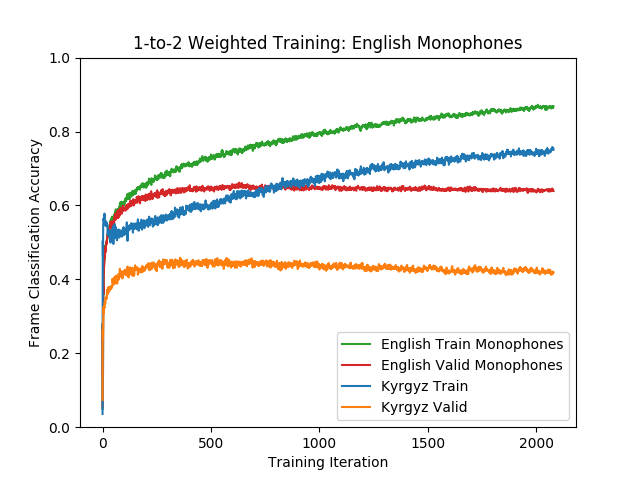
\includegraphics[width=1.1\textwidth,keepaspectratio]{figs/1-to-2-mono.png}
  \caption{Aux Task = Monophones}
  \label{fig:sub1}
\end{subfigure}%
\begin{subfigure}{.25\textwidth}
  \centering
  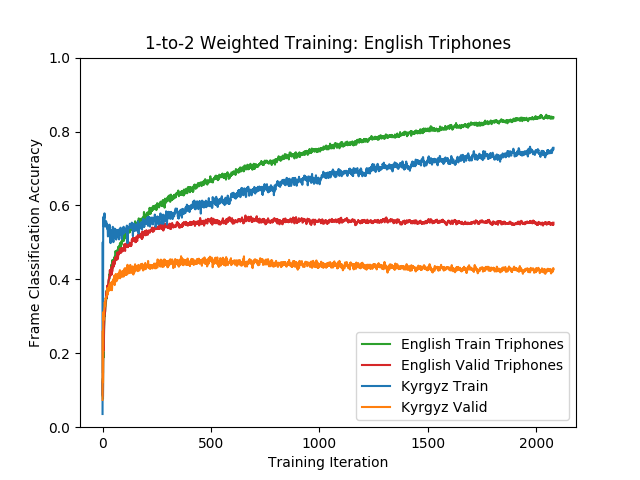
\includegraphics[width=1.1\textwidth,keepaspectratio]{figs/1-to-2-tri.png}
  \caption{Aux Task = Triphones}
  \label{fig:sub2}
\end{subfigure}
\caption{1-to-2 Weighted MTL Training | Kyrgyz and English Classification Accuracy}
\label{fig:1-to-2}
\end{figure}


Firstly, let's compare two models which were trained with the same 1-to-2 (target-to-source) weighting scheme, but different levels of abstraction (ie. monophones vs triphones). We see that the performance on English training data (in Green) is better than performance on Kyrgyz training data (in Blue). This is the case for both the monophone and triphone model. Also we see that the model generalizes better for English than for Kyrgyz (ie. English validation (Red) is always better than Kyrgyz validation (Orange)).

In general, our aim is to increase the Kyrgyz validation performance (Orange). We can take away from these graphs a few things. Firstly, looking at the performance on English at this weighting scheme, performance on monophone train is higher than on triphone train. Both models clearly overfit, with validation performance plateauing after about 500 iterations, but monophone classification reaches over 60\% accuracy vs. under 60\% accuracy for triphones. This makes sense, because the model has around 1500 labels for train and only around 200 for monophones.




Taking a look at the 2-to-1 weighting scheme in Figure (\ref{fig:2-to-1}), where the Kyrgyz data has more importance during backprop, we see a very different picture.


\begin{figure}[!htbp]
\centering
\begin{subfigure}{.25\textwidth}
  \centering
  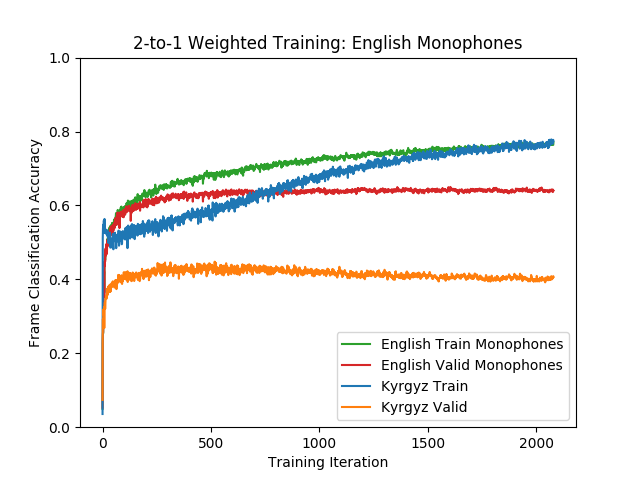
\includegraphics[width=1.1\textwidth,keepaspectratio]{figs/2-to-1-mono.png}
  \caption{Aux Task = Monophones}
  \label{fig:sub1}
\end{subfigure}%
\begin{subfigure}{.25\textwidth}
  \centering
  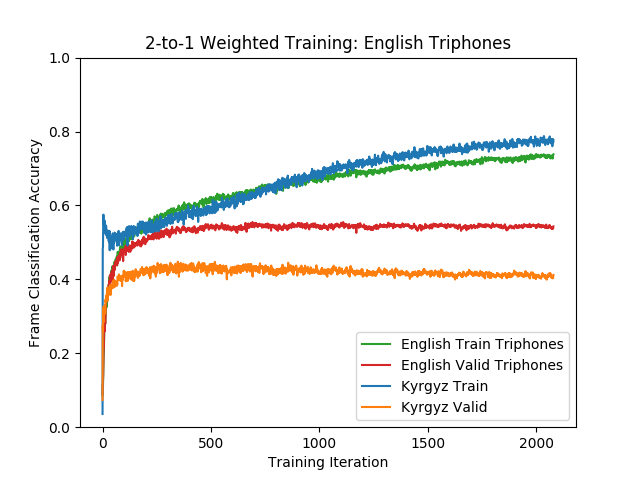
\includegraphics[width=1.1\textwidth,keepaspectratio]{figs/2-to-1-tri.png}
  \caption{Aux Task = Triphones}
  \label{fig:sub2}
\end{subfigure}
\caption{2-to-1 Weighted MTL Training | Kyrgyz and English Classification Accuracy}
\label{fig:2-to-1}
\end{figure}


We can see that even though the Kyrgyz data is more heavily weighted, the English monophones quickly overfit. However, the shared hidden layers clearly favor the Kyrgyz data, and the model fits to Kyrgyz more rapidly than it does to English. The weight eventually overfit to both models equally.

Looking over at the performance of the model trained with English triphones as an auxiliary task, we find that not the model fits the Kyrgyz training data, but by the end of 2000 iterations (10 epochs), the weights have found a local minimum which is better for Kyrgyz than English. The influence of the English triphones during backprop is too diffuse to steer the hidden layer weights in direction favorable to the auxiliary task, English.


\section{Conclusions}

Multi-Task Learning promises a very simple solution to a very hard problem. It would seem that as long as we can add relevant tasks to our net, through the good graces of backprop, a best solution will automatically be discovered. It would also seem that we are guaranteed to get better results as long as we keep adding related tasks. This study shows that the picture is not so simple.

Starting with three additional tasks, which are clearly related \textit{a priori}, the current study investigated not only their relative import, but also the dynamics of their combinations. Each task represented a level of abstraction from the typical training labels, from fine-grained (triphones), to more abstract (half-phones) to completely context-free (monophones). In addition to these three levels (deduced from a given decision tree), I tested logical combinations of abstractions: the entire tree, the top half of the tree, and the bottom half of the tree. None of these combinations outperformed the tasks added individually.

Discussed more deeply than the results of combinations of tasks was the performance of the tasks with regards to differential weighting and their level of abstraction. Their level of abstraction correlates to number of labels in the task, and as such number of nodes in the output layer, and as such number of parameters in the model.

With more labels, the task is inherently more difficult and the model has more parameters to train. As such, models with fewer labels found their local minimum more quickly, and were less likely to succeed influence over shared hidden layers to another task (ie. Kyrgyz).

If a task is simple, the net will find a good local minimum quickly. As such, in MTL setups, care should be taken to weighting auxiliary tasks relative to their simplicity.

Hard tasks exert less of an influence on other tasks, but simple tasks can dominate during training. As such, care must be taken to weight accordingly, even if tasks are related.




\section{Acknowledgements}

I'd like to thank Dan Povey for answering my (oftentimes naive) questions on the kaldi-help Google Group.

I'd like to also thank Chorobek Saadanbekov and Murat Jumashev for making the Kyrgyz audiobook available to me through the Bizdin.kg group.

This material is based upon work supported by the National Science Foundation Graduate Research Fellowship under Grant No. (DGE-1746060). Any opinion, findings, and conclusions or recommendations expressed in this material are those of the authors(s) and do not necessarily reflect the views of the National Science Foundation.

\newpage

\bibliographystyle{IEEEtran}
\bibliography{mybib}



\end{document}
